% !TeX root = ./main.tex
We will validate the gain in efficiency and quality of using the proposed Optimal Unsatisfiable Subset detection algorithms for explaining satisfiable constraint satisfaction problems.

We consider the following benchmarks: CNF instances \tias{Emilio:...} from \tias{Emilio:...} and a CNF encoding of the logic grid puzzle used in~\cite{ecai/BogaertsGCG20}. All code was implemented in Python on top of %CPpy~\footnote{} and
PySAT~\footnote{\url{https://pysathq.github.io}}. The MIP solver used is Gurobi 9.0 and when a MaxSAT solver is used it is RC2 as bundled with PySAT. Experiments were run on a \tias{Emilio:...}

We aim to answer the following research questions:
\begin{itemize}
\item RQ1: what is the effect of delaying propagation, incremental OUS solving and pre-seeding the MCS when solving multiple variants of the same problem?
\item RQ2: how do the different variants perform when explaining an elaborate constraint satisfaction problem?
\item RQ3: how do the sequences found when using (constrained) OUS search compare to those found using a heurisic MUS approach?
\end{itemize}

\paragraph{RQ1}
To answer the first research question, we collected a number of CNF instances from \tias{Emilio:...}. We randomly choose a subset of 10 decision variables and a fixed ordering among them, and then compare the following variants: 1) 2) 3)... \tias{Emilio:...}

The results can be seen in Table \tias{Emilio:...} and can be summarized as follows: \tias{Emilio:...}


\paragraph{RQ2}
The second research question is how do the different variants perform when explaining an elaborate constraint satisfaction problem? The results for the logic grid puzzle called 'origin' is shown in Figure~\ref{fig:exp2}.

\begin{figure}[t]
    \centering
    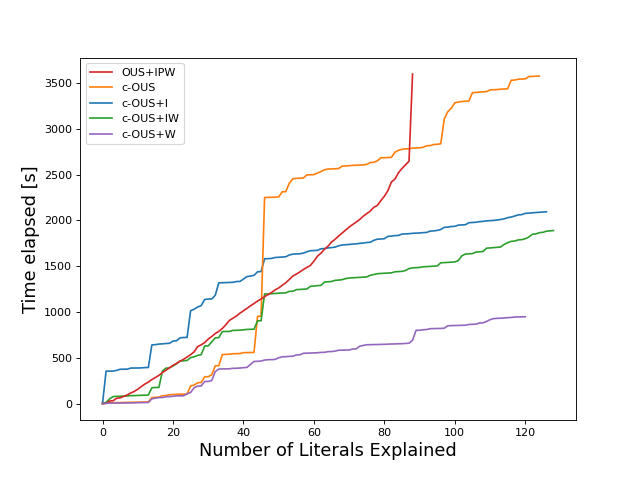
\includegraphics[width=\columnwidth]{figures/omusConstrCumulative.png}
    \caption{Experiment 2}
    \label{fig:exp2}
\end{figure}

The figure shows the number of literals explained on the X-axis, and the cumulative time taken on the X-axis. 
We can see that OUS-Incremental with pre-seeding and post-poning optimisation is not able to explain all of the literals within the timeout; especially around step 95 there is a big jump in runtime. The vanilla constrained-OUS approach is not able to finish in time either, with big jumps in time on specific (hard) clues.

When combining constrained-OUS with either pre-seeding, post-poned optimisation or both, then our approach is able to fully explain the solution. Best results are obtained with constrained-OUS with just pre-seeding at the beginning. The post-poned optimisation in this case may spent a lot of time generating MCSs that are not or little relevant to the constrained OUSs we are seeking.

Finally, for \textbf{RQ3} we compare the sequence found by our proposed method with the sequence reported on in~\cite{ecai/BogaertsGCG20} for the origin puzzle. \tias{Emilio: ...}


%
%\begin{figure*}[ht]
%    \centering
%    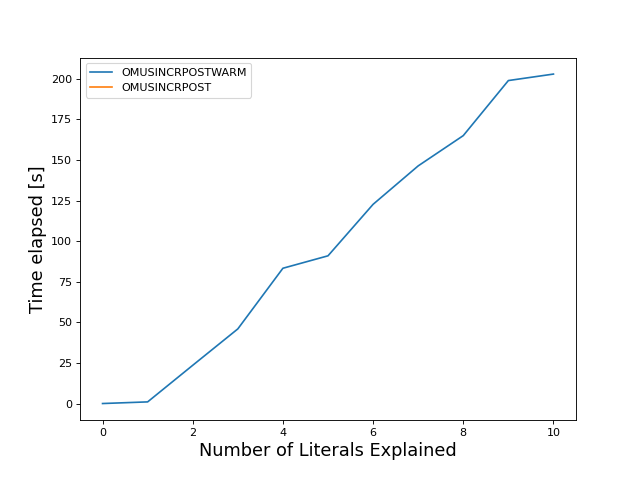
\includegraphics[width=\columnwidth]{figures/omusNonConstrCumulative.png}
%    \caption{}
%    \label{}
%\end{figure*}

\begin{figure}[ht]
    \centering
    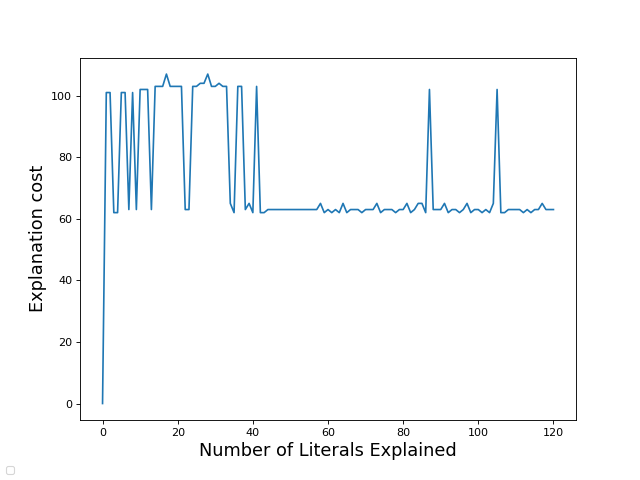
\includegraphics[width=\columnwidth]{figures/explanation_cost.png}
    \caption{}
    \label{}
\end{figure}

